Throughout the input specification the user is defining variables. As
described in the above sections many of these variables can be
specified by the user to be random variables with a distribution on
their values. It is in the UQ panel that the user specifies what these
distributions are.
It is also here that the user specifies the UQ method and the input
values are for these UQ methods.  The panel is split, as shown
in \Cref{fig:figure10}, into 2 frames:

\begin{enumerate}
\item Sampling Methods 
\item Random Variables
\end{enumerate}

\begin{figure}[!htbp]
  \centering {
    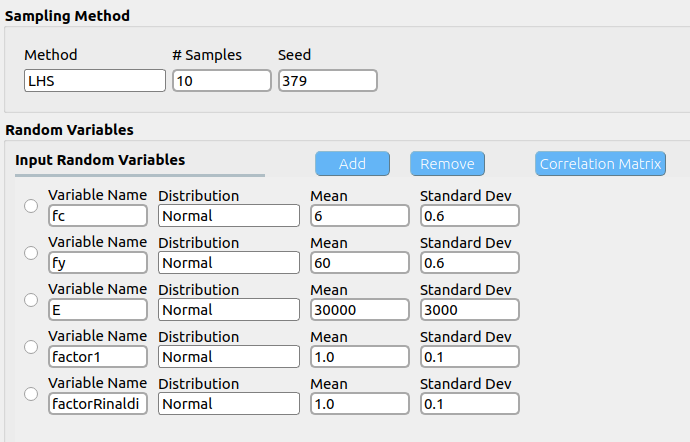
\includegraphics[width=0.8\textwidth]
    {usage/figures/uq1.png} }
  \caption{Uncertainty Quantification input panel}
  \label{fig:figure10}
\end{figure}

\subsection{Sampling Methods}
In the \href{https://dakota.sandia.gov//sites/default/files/docs/6.9/html-ref/methods-sampling.html}{sampling methods} the user selects the sampling 
method to use from the method dropdown. Currently this is limited to 
two options: Monte Carlo and Latin Hypercube Sampling (LHS). For the 
one selected, the user specifies the number of simulations to be 
perform and the seed.

\subsection{Random Variables}
The Random Variable panel is where the user enters the random
variables. Each random variable has a name and a distribution. The
distribution is selected from the drop-down menu. By changing the
distribution type, the inputs required to define the distribution
change. The following are the list of distributions available (clicking on any link will take you to Dakota manual explaining inputs and theory):
\begin{enumerate}
\item \href{https://dakota.sandia.gov//sites/default/files/docs/6.9/html-ref/variables-normal_uncertain.html}{Normal}
\item \href{https://dakota.sandia.gov//sites/default/files/docs/6.9/html-ref/variables-lognormal_uncertain.html}{Lognormal}
\item \href{https://dakota.sandia.gov//sites/default/files/docs/6.9/html-ref/variables-beta_uncertain.html}{Beta}
\item \href{https://dakota.sandia.gov//sites/default/files/docs/6.9/html-ref/variables-uniform_uncertain.html}{Uniform}
\item \href{https://dakota.sandia.gov//sites/default/files/docs/6.9/html-ref/variables-weibull_uncertain.html}{Weibull}
\item \href{https://dakota.sandia.gov//sites/default/files/docs/6.9/html-ref/variables-gumbell_uncertain.html}{Gumbell}
\end{enumerate} 

As with other panels, the random variables can be added or
removed. Care must be taken by the user in ensuring that if the user
removes random variables from this panel that they also remove them
from the other input widgets. Failing to do so may result in the
program failing to complete.
